\chapter{Аналитическая часть}

\section{Описание объектов сцены}

Сцена состоит из источника света, молнии, дома и плоскости земли.
Источник свет представляет собой материальную точку, испускающую лучи света во все стороны (если источник расположен в бесконечности, то он имеет направление). В моей программе источником света будет молния.
Молния представляет собой ломаную линию, которая имеет начало и конец, а также несколько ветвей. 
Дом – сооружение, для которого пользователь должен задать этажность, а также указать, в каких окнах включен свет.
Плоскость земли – это некая ограничивающая плоскость. Предполагается, что под такой плоскостью не расположено никаких объектов. Располагается на максимальной координате по оси У. 


\section{Анализ и выбор формы задания трехмерных моделей}

Отображением формы и размеров объектов являются модели. 
Обычно используются три формы задания моделей.

\begin{enumerate}
	\item Каркасная (проволочная) модель.
	
	Одна из простейших форм задания модели, так как мы храним информацию только о вершинах и ребрах нашего объекта. Недостаток данной формы состоит в том, что модель не всегда точно передает представление о форме объекта.
	
	\item Поверхностная модель.
	
	Такой тип модели часто используется в компьютерной графике. Поверхности можно задавать разными способами: либо аналитически, либо задавать участки поверхности, как поверхность того или иного вида (использовать полигональную аппроксимацию). Недостаток данной формы состоит в том, что мы не знаем с какой стороны находится материал.
	
	\item  Объемная (твердотельная) модель.
	
	Данная форма отличается от поверхностной тем, что у нас есть информация о том, где расположен материал. Это делается с помощью указания направления внутренней нормали. 
	Таким образом, можно сделать вывод о том, что для решение данной задачи нам подойдут поверхностные модели, так как каркасные модели могут привести к неправильному восприятию формы, а объемные модели будут излишеством, так как будут тратить больше памяти.
\end{enumerate}


\subsection{Анализ способа задания поверхностных моделей}

Также необходимо определить каким образом лучше всего задавать поверхностные модели.

\begin{itemize} 
\item Аналитическим способом. Этот способ задания модели характеризуется описанием модели объекта, которое доступно в неявной форме, то есть для получения визуальных характеристик необходимо дополнительно вычислять некоторую функцию, которая зависит от параметра.

\item Полигональной сеткой. Данный способ характеризуется совокупностью вершин, граней и ребер, которые определяют форму многогранного объекта в трехмерной компьютерной графике.

\end{itemize}


Для более верного выбора также следует перечислить способы хранения информации о сетке.

\begin{itemize}

\item Список граней. Объект – это множество граней и множество вершин. В каждую грань входят как минимум 3 вершины;
\item«Крылатое» представление. Каждая точка ребра указывает на две вершины, две грани и четыре ребра, которые её касаются;
\item Полурёберные сетки. То же «крылатое» представление, но информация обхода хранится для половины грани;
\item Таблица углов. Таблица, хранящая вершины. Обход заданной таблицы неявно задаёт полигоны. Такое представление более компактно и более производительно для нахождения полигонов, но, в связи с тем, что вершины присутствуют в описании нескольких углов, операции по их изменению медленны.
\item Вершинное представление. Хранятся лишь вершины, которые указывают на другие вершины. Простота представления даёт возможность проводить над сеткой множество операций.

\end{itemize}


Стоит отметить, что одним из решающих факторов в выборе способа задания модели в данном проекте является скорость выполнения преобразований над объектами сцены.

При реализации программного продукта наиболее удобным представлением является модель, заданная полигональной сеткой – это поможет избежать проблем при описании сложных моделей. При этом способ хранения полигональной сетки – список граней, так как он предоставляет явное описание граней, что поможет при реализации алгоритма удаления невидимых рёбер и поверхностей. Также этот способ позволит эффективно преобразовывать модели, так как структура будет включать в себя список вершин. 



\section{Анализ и выбор алгоритма удаления невидимых ребер и поверхностей}

Перед выбором алгоритма удаления невидимых ребер выделим несколько свойств, которыми должен обладать выбранный алгоритм, чтобы обеспечить оптимальную работу и реалистичное изображение.

Свойства:	
\begin{itemize}
\item	алгоритм может работать как в объектном пространстве, так и в пространстве изображений;
\item	алгоритм должен быть достаточно быстрым и использовать мало памяти;
\item	алгоритм должен иметь высокую реалистичность изображения.
\end{itemize}

\subsection{Алгоритм, использующий Z-буфер}

\subsection{Алгоритм обратной трассировки лучей}

Суть данного алгоритма состоит в том, что наблюдатель видит объект с помощью испускаемого света, который согласно законам оптики доходит до наблюдателя некоторым путем. Отслеживать пути лучей от источника к наблюдателю неэффективно с точки зрения вычислений, поэтому наилучшим способом будет отслеживание путей в обратном направлении, то есть от наблюдателя к объекту.

Положительными моментами в этом алгоритме являются:
\begin{itemize}
\item	высокая реалистичность синтезируемого изображения;
\item	работа с поверхностями в математической форме;
\item	вычислительная сложность слабо зависит от сложности сцены.
\end{itemize}

Недостаток:
\begin{itemize}
\item	производительность.
\end{itemize}
Вывод

Данный алгоритм не отвечает главному требованию – скорости работы, но при некоторой адаптации можно добиться большей скорости работы. 



\subsection{Алгоритм Робертса}



\begin{equation} 
	\label{for:qint}
	\Psi = \sum\limits_{\overrightarrow{i}=\ket{00...0}}^{\overrightarrow{i} = \ket{11...1}} A \rightarrow_{i} \Psi(\ket{\overrightarrow{i}})
\end{equation}


\subsection{Алгоритм художника}

Данный алгоритм работает аналогично тому, как художник рисует картину – то есть сначала рисуются дальние объекты, а затем более близкие. Наиболее распространенная реализация алгоритма – сортировка по глубине, которая заключается в том, что произвольное множество граней сортируется по ближнему расстоянию от наблюдателя, а затем отсортированные грани выводятся на экран в порядке от самой дальней до самой ближней. Данный метод работает лучше для построения сцен, в которых отсутствуют пересекающиеся грани. 

Положительным моментом данного алгоритма является:
\begin{itemize}
\item	требование меньшей памяти, чем, например, алгоритм Z-буффера.
\end{itemize}

Недостатки

\begin{itemize}
\item	недостаточно высока реалистичность изображения;
\item	сложность реализации при пересечения граней на сцене.
\end{itemize}

Вывод

Данный алгоритм не отвечает главному требованию – реалистичность изображения. Также алгоритм художника отрисовывает все грани (в том числе и невидимые), на что тратится большая часть времени.


\subsection{Алгоритм Варнока}

 Алгоритм Варнока является одним из примеров алгоритма, основанного на разбиении картинной плоскости на части, для каждой из которых исходная задача может быть решена достаточно просто.
 
 Поскольку алгоритм Варнока нацелен на обработку картинки, он работает в пространстве изображения. В пространстве изображения рассматривается окно и решается вопрос о том, пусто ли оно, или его содержимое достаточно просто для визуализации. Если это не так, то окно разбивается на фрагменты до тех пор, пока содержимое фрагмента не станет достаточно простым для визуализации или его размер не достигнет требуемого предела разрешения.
 
 Сравнивая область с проекциями всех граней, можно выделить случаи, когда изображение, получающееся в рассматриваемой области, определяется сразу:
 
\begin{itemize}
 \item	проекция ни одной грани не попадает в область;
\item	проекция только одной грани содержится в области или пересекает область, то в этом случае проекции грани разбивают всю область на две части, одна из которых соответствует этой проекции;
\item	существует грань, проекция которой полностью накрывает данную область, и эта грань расположена к картинной плоскости ближе, чем все остальные грани, проекции которых пересекают данную область, то в данном случае область соответствует этой грани.
\end{itemize}
 
 Если ни один из рассмотренных трех случаев не имеет места, то снова разбиваем область на четыре равные части и проверяем выполнение этих условий для каждой из частей. Те части, для которых таким образом не удалось установить видимость, разбиваем снова и т. д.
 
 Преимущества:
 
\begin{itemize}
\item	меньшие затраты по времени в случае области, содержащий мало информации.
\end{itemize}

 Недостатки:
 \begin{itemize}
\item	алгоритм работает только в пространстве изображений;
\item	большие затраты по времени в случае области с высоким информационным содержимым.
\end{itemize}

 Вывод
 
 Данный алгоритм не отвечает требованию работы как в объектном пространстве, так и в пространстве изображений, а также возможны большие затраты по времени работы.
 
 
\subsection*{Вывод}

Для удаления невидимых линий выбран алгоритм обратной трассировки лучей. Данный алгоритм позволит добиться максимальной реалистичности и даст возможность смоделировать распространение света в пространстве, учитывая законы геометрической оптики. Данный алгоритм можно модернизировать, добавив в него обработку новых световых явлений. Также этот алгоритм позволяет строить качественные тени с учетом большого числа источников. Стоит отметить тот факт, что алгоритм трассировки лучей не требователен к памяти, в отличие, например, от алгоритма Z-буфера.

\subsection{Квантовая фазовая логика}

Квантовая фазовая логика инвертирует фазу каждого входного значения, которое дает 1 в результате.
Фазовая логика принципиально отличается от любой традиционной логики -- результаты логических операций скрыты в фазах и их невозможно прочитать. Но, при этом, инвертируя фазы в суперпозиции, можно пометить несколько решений в одном регистре. Кроме того, при использовании инвертирования и усиления комплексной амплитуды можно создавать результаты, доступные для чтения.

С помощью комбинации усилении амплитуды и операций фазовой логики, можно сохранить значение логической операции в фазе состояния \cite{PQC-logic}. Таким образом, мы можем описывать более сложные фигуры, например кривые.

Окружность задается уравнением вида (\ref{for:circle}):

\begin{equation}
	\label{for:circle}
	x^2 + y^2 = r^2
\end{equation}

Предположим, что мы хотим заполнить все пиксели, находящиеся внутри окружности, то есть пиксели, подходящие под условие (\ref{for:circle2}):

\begin{equation}
	\label{for:circle2}
	x^2 + y^2 < r^2
\end{equation}

Для выполнения этого действия нам потребуются выше описанные регистры $qx$ и $qy$, а так же дополнительные регистр-аккумулятор $qacc$. Дальнейший алгоритм таков:

\begin{itemize}
	\item инициализировать регистры $qx$, $qy$ и $qacc$;
	\item ввести регистры $qx$ и $qy$ в суперпозицию;
	\item добавить в регистр $qacc$ сумму квадратов регистров $qx$ и $qy$;
	\item вычесть из регистра $qacc$ квадрат радиуса описываемой окружности;
	\item инвертировать регистр $qacc$ для всех значащих битов;
	\item восстановить регистр $qacc$.
\end{itemize}

\begin{figure}[h]
	\begin{center}
		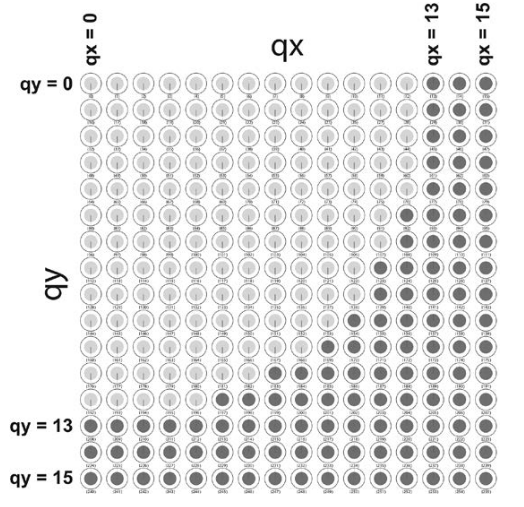
\includegraphics[scale=0.57]{img/holst_03.png}
	\end{center}
	\captionsetup{justification=centering}
	\caption{Переключение кривых на холсте с помощью фазовой логики.}
	\label{for:holst_03}
\end{figure}

\subsection{Квантовое преобразование Фурье}\label{furie}

Квантовое преобразование Фурье позволяет обращаться к скрытой информации, хранящейся в фазах и амплитудах квантового регистра. Данный примитив предоставляет собственный механизм манипуляций с фазами кубитов \cite{PQC-furie}).

Допустим, имеется четырехкубитный квантовый регистр, содержащий одно из трех состояний, но точно неизвестно какое (рисунок \ref{img:furie-example-01}). Как уже говорилось ранее, при чтении регистра будет полученно случайное значение с равномерным распределением. 

\begin{figure}[h]
	\begin{center}
		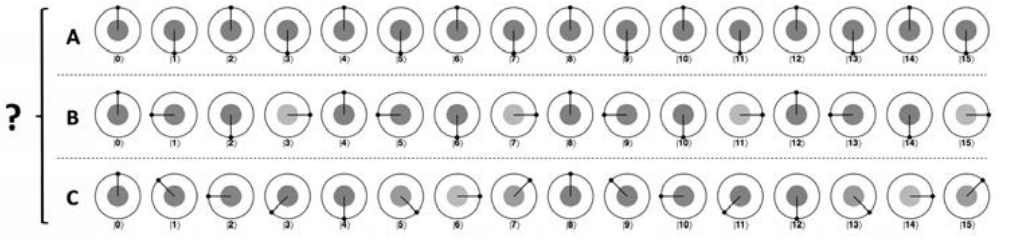
\includegraphics[scale=0.4]{img/furie-example.png}
	\end{center}
	\captionsetup{justification=centering}
	\caption{Три разных состояние кубита до применения квантового преобразования Фурье}
	\label{img:furie-example-01}
\end{figure}

Усиление квантовой амплитуды в данном примере не принесет никакой пользы, так как нет какой-то одной фазы, которая бы выделялась на фоне других в каждом состоянии. Применение квантового преобразования Фурье к рассматриваемому регистру перед чтением результата преобразует каждое из состояний к результату, показанному на рисунке \ref{img:furie-example-02}. Таким образом, можно однозначно определить, какое состояние было исходным.

\begin{figure}[h]
	\begin{center}
		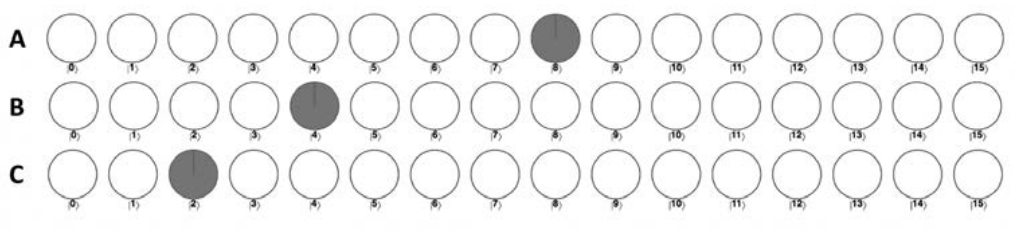
\includegraphics[scale=0.4]{img/furie-example-02.png}
	\end{center}
	\captionsetup{justification=centering}
	\caption{Три разных состояние кубита после применения квантового преобразования Фурье}
	\label{img:furie-example-02}
\end{figure}

Между результатами на рисунке \ref{img:furie-example-01} можно заметить связь: в первом состоянии фаза входного состояния возвращается в 0 восемь раз, а квантовое преобразование Фурье позволяет прочитать значение 8. Во втором состоянии  фаза возвращается к своему начальному состоянию четыре раза, а квантовое преобразование Фурье позволяет прочитать значение 4. Третье состояние подчиняется той же самой закономерности. Квантовое преобразование Фурье успешно открывает частоту сигнала \cite{signal}, содержащуюся в квантовом регистре. Само по себе квантовое преобразование Фурье имеет сильное сходство с классическим механизмом обработки сигналов, называемым дискретным преобразованием Фурье \cite{PQC-furie-proof}.

\section{Квантовая избыточная выборка}

Избыточная выборка -- процесс увеличения число дискретных выборок на пиксель. На один пиксель проецируется не один, а несколько лучей. Результат проекции каждого такого луча сохраняется в соответствующий субпиксель (англ. subpixel). После того, как все нужные выборки сохранены в экранном буфере, итоговый цвет пикселя определяется как усреднённый цвет всех соответствующих ему субпикселей. Таким образом, формула принимает вид (\ref{for:supersampling}): 

\begin{equation}
	\label{for:supersampling}
	res = \frac{sample_{0} + sample_{1} + ... + sample_{n-1}}{n} = \frac{\sum_{i=0}^{n - 1} sample_{i}}{n}
\end{equation}

где:

\begin{itemize}
	\item $res$ -- итоговый цвет пикселя;
	\item $n$ -- количество выборок на пиксель;
	\item $sample_{i}$ -- цвет $i$-ой выборки.
\end{itemize}

В случае квантовой избыточной выборки, для каждого блока необходимо оценить количество субпикселов с инвертированной фазой. Для черных и белых субпикселов (представленных инвертированной или не инвертированной фазой) это позволит нам получить значение для каждого результирующего пиксела, характеризующее интенсивность исходных составляющих субпикселов.

Преимущества использования квантовой избыточной выборки (по сравнению с обычной) связано не с количеством операций графического вывода, а с различиями в характере наблюдаемого шума. В среднем, при сравнении двух идентичных синтезируемых изображения, погрешность на пиксель у квантовой избыточной выборки на 33\% ниже, чем у метода Монте-Карло (обычная избыточная выборка) \cite{PQC-prcnt}. Помимо этого, количество пикселов с нулевой погрешность в среднем в два раза больше, чем у метода Монте-Карло \cite{PQC-prcnt}.

\subsection{Принцип работы}

Основополагающая идея квантовой избыточной выборки заключается в применении метода объединения итераций усиления комплексной амплитуды (\ref{yka}) с квантовым преобразованием Фурье (\ref{furie}). Квантовое преобразование Фурье позволит оценить количество элементов, инвертированных квантовой логикой, используемой в подсхеме инвертирования каждой итерации усиления комплексной амплитуды. В данном случае подсхемой инвертирования является программа, которая инвертирует фазу белых субпикселей.

Определим квантовый регистр, который будет выполнять роль <<счётчика>>. Значение этого регистра будет определять, сколько итераций выполнит наша схема. Введя регистр в суперпозицию, будет выполнено суперпозиция разного количества итераций усиления комплексной амплитуды. Как уже было написано выше, вероятность чтения нескольких инвертированных значений в регистре зависит от количества выполняемых итераций. Кроме этого, колебания вводятся в зависимости от количества инвертированных значений. Таким образом, при выполнении суперпозиции разного количества итераций усиления комплексной амплитуды, вводятся периодические колебания по комплексным амплитудам квантового регистра с частотой, зависящей от количества инвертированных значений.

Для чтения частот, закодированных в квантовых регистра, можно использовать квантовое преобразование Фурье \cite{PQC-fourier}. Зная количество субпикселей, использованных в квантовой выборке, можно определить яркость анализируемого пикселя.

Качество выборки напрямую зависит от количества кубитов для <<счётчиков>>. С увеличением количества образцов (кубитов) вероятность получения точного ответа растёт \cite{PQC-qbits}.

\subsection{Поисковая таблица}\label{table-q}

При запуске квантового алгоритма избыточной выборки и в конце его выполнения читая значение квантового регистра, мы получаем число -- оно связано с количеством белый субпикселей в заданном блоке, но не будет точно равно ему. 

Поисковая таблица квантовой выборки (англ. quantum supersamping lookup table) -- инструмент для определения количества субпикселей в блоке, подразумеваемого считанным значением из квантового регистра. Например, поисковая таблица, для квантовой выборки с размером квантового шейдера $4x4$ и регистром счетчиком, состоящим из четырех кубитов, будет выглядить как таблица с $2^4 = 16$ столбцами и $2^4 = 16$ строками. В строках поисковой таблицы перечисляются возможные результаты чтения значения из квантового регистра. В столбцах перечисляются возможные количества  субпикселей в квантовом шейдере, которые могут привести к такому значению, который был получен путём чтения квантового регистра.

При получении значения из квантового регистра, в поисковой таблице выбирается строка соответствующая считанному значению. Далее, оценивая количество <<белых>> субпикселей, расположенные в этой строке (а точнее лишь вероятность нахождения этих субпикселей в анализируемом пикселе), выбирается конечная яркость пикселя. Из-за того что в строчках расположенны лишь вероятности, появляется некоторая погрешность и не всегда можно  однозначно определить яркость пикселя.

Таким образом, можно описать функцию, на вход принимающую номер строки ($k$) таблицы, и возвращающую вероятность яркости пикселя (\ref{for:table_function}):

\begin{equation}
	\label{for:table_function}
	\gamma(k) = \sum_{i=0}^{n - 1} x_{k_i}
\end{equation}


Поисковая таблица -- характерный признак алгоритма квантовой избыточной выборки. С увеличением размера квантового шейдера (следовательно увеличения количества субпикселей), растёт вероятность точного определения яркости выбранного пикселя.

\begin{figure}[H]
	\begin{center}
		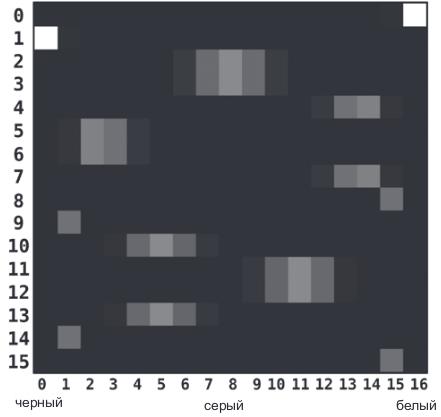
\includegraphics[scale=0.55]{img/qss_table.png}
	\end{center}
	\captionsetup{justification=centering}
	\caption{Поисковая таблица квантовой выборки. По оси OY -- результат квантовой выборки, по оси OX -- цвет пикселя (сумма белых пикселей)}
	\label{img:qss_table}
\end{figure}

\subsection{Карта достоверности}\label{map}

Поисковая таблица также может использоваться для получения вероятности того, что итоговая яркости пиксела выбрана правильно. По расположению считанного значения из квантового регистра, в строке таблицы можно оценить вероятность того, что полученное значение было правильным. Для каждого значения из выбранной строки имеется вероятность что данный субпиксель является белым -- это можно сделать с помощью расположения считанного значения (в процессе избыточной выборки) в соответствующей строке таблице поиска. По этим результатам можно построить <<карту достоверности>> (англ. confidence map), обозначающую вероятное расположение ошибок в синтезируемом изображении.

\begin{figure}[H]
	\begin{center}
		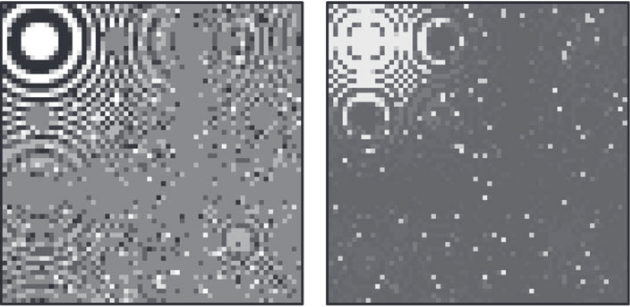
\includegraphics[scale=0.6]{img/map.png}
	\end{center}
	\captionsetup{justification=centering}
	\caption{Карта достоверности. Слева -- результат квантовой выборки, справа -- карта достоверности на уровне пикселей.}
	\label{img:map}
\end{figure}

\section{Колоризация изображения}\label{color}

Фазы и комплексные амплитуды квантового регистра можно использовать для кодирования более широкого диапазона цветовых значений (помимо белого и черного), но тогда метод квантовой избыточной выборки работать не будет \cite{PQC-color}. 

Для колоризации изображения можно воспользоваться технологией битовых слоёв. Квантовый пиксельный шейдер будет использоваться для построения отдельных монохромных изображений, каждое из которых будет представлять один бит изображения. Таким образом, пиксельный шейдер фактически будет генерировать $N$ монохромных изображений, где $N$ -- количество цветов, которые нужно <<запутать>> в изображении. Все эти $N$ изображений пройдут квантовую избыточную выборку по отдельности и будут объединены в итоговое цветное изображение.

\section*{Вывод}

В данном разделе был проведен анализ квантовых алгоритмов и структур данных, которые возможно использовать в поставленной задаче. В качестве ключевого алгоритма, который может улучшить качество синтезируемого изображения, выбран алгоритм квантовой избыточной выборки, в сочетании с такими структурами данных как квантовая поисковая таблица и квантовая карта достоверности. Именно этот алгоритм и будет реализован в рамках данной работы.